\documentclass[12 pt]{scrartcl}
\usepackage{setspace}
\usepackage{url}
\onehalfspacing
\usepackage{amsmath,amssymb,amsfonts,amsthm,mathtools}
\usepackage[english]{babel}
\usepackage[T1]{fontenc}
\usepackage[utf8x]{inputenc}
\usepackage{lmodern}
\usepackage{dsfont}
\usepackage{bbm}
\usepackage[round]{natbib}
\usepackage{color} 
\usepackage[defaultlines=2,all]{nowidow}
\usepackage{caption}
\usepackage[labelformat=simple]{subcaption}
\usepackage{makecell}
\renewcommand\thesubfigure{(\alph{subfigure})}

\setlength\parindent{0pt}
\setlength{\parskip}{6pt plus 1pt minus 1pt}

\newcommand{\red}{\textcolor{red}}


\begin{document}

\begin{titlepage}
  \centering
  {\scshape\LARGE TU Dortmund \par}
  \vspace{1cm}
  {\scshape\Large Introductory Case Studies \par}
  \vspace{2cm}
  {\huge\bfseries Project 3: Regression analysis for price of VW cars\par}
  \vspace{2cm}
  {\Large Lecturers:\\
    Prof.\ Dr.\ Sonja Kuhnt\\
    Dr.\ Paul Wiemann\\
    Dr.\ Birte Hellwig\\
    M.\ Sc.\ Hendrik Dohme \par}
  \vspace{1cm}
  {\Large Author: Tadeo Hepperle \par}
  \vspace{0.5 cm}
  {\Large Group number: 2\par}
  \vspace{0.5 cm}
  {\Large Group members: Prem Kant Shekhar, Minjae Ok, Ishan Singh Dhapola, Fyalisia Amanda Putri, Tadeo Hepperle}
  \vfill
  {\large \today\par}
\end{titlepage}


\tableofcontents

\cleardoublepage

\section{Introduction}

Every year millions of cars are bought and sold around the globe. Despite the pandemic, 2.62 million cars newly registered in Germany in the year 2020, according to \citet{Statisti39}.
Almost 10\% of Germany's GDP comes from automobile companies and their suppliers. About 930,000 people work in the German car industry \citep{dw}.
The massive size of this economic sector and its impact on our daily life makes it important to talk about the prices of cars. Purchased for 36,300 EUR on average \citep{Statista2}, cars can lose their value pretty quickly. Therefore many consumers rather buy used cars. According to \citet{Handelsblatt}, about 2 out of three newly registered cars are not new. Therefore in this report we will look at the prices of used cars sold on the british car internet platform "Exchange and Mart" \citep{Exchangeandmart}. Our dataset contains prices and predictors such as age, tax, mileage, transmission type, fuel type  fuel consumption and engine size for 438 VW cars of the 3 popular models Passat, Up and T-Roc. Our goal is to predict the price of a car as accurately as possible using the variables mentioned. For this we are using multiple linear regression on the logarithmic price as the variable we want to predict, because the data suggests that the logarithmic price can be better modeled using the predictors. After conducting best subset selection we found that a regression model containing the six predictor variables car model, age, mileage, transmission type, engine size and fuel type was best at predicting the price of VW cars. More than 96 percent of the variation in the price of a car was rooted in these variables. Overall we found that greater mileage and age reduce a cars price while higher engine size increases it. Hybrid cars sell for much more than Petrol and Diesel cars, while automatic transmission gets you a higher price tag on your car as well.
There were also huge differences between the different models.
In section 2 the goals of the report are outlined and we explain the VW cars data set in detail, while the statistical methods around multiple linear regression are explained in section 3. Section 4 holds the results and as a part of that the final model with all its coefficients. These are interpreted properly to reveal their meaning to the untrained eye. Finally section 5 summarizes the project and its implications for what to consider when looking for buying or selling a used car.

\section{Problem statement}

We analyzed a data set containing prices and other features of 438 cars from the german car brand VW to determine which factors influence the price of a car and to what extent they do so. This makes it possible to predict the value of a car by knowledge about its features.

\subsection{Description of the dataset}

The dataset used in this report is a sclice of a bigger dataset from kaggle.com and contains data about 438 VW cars, which were originally scraped in 2020 from the british car internet platform "Exchange and Mart" \citep{Exchangeandmart}
(https://www.exchangeandmart.co.uk/). The slicing was done to only include the VW models "Passat", "T-Roc" and "Up".
For each of the 438 cars information on the following variables is provided:
\begin{itemize}
  \item the \textbf{price} a car is selling for in 1000 GBP (£)
  \item the \textbf{year} a car was first registered
  \item the \textbf{mileage} as the total distance a car has been driven in 1000 miles
  \item the \textbf{fuel consumption} in mpg, the number of miles a car can drive with one gallon of fuel
  \item the \textbf{fuel type} a car uses, categorical variable with 3 levels: "Diesel", "Hybrid", "Petrol"
  \item the \textbf{engine size} as the volume of fuel in liters and air a car can fit in its engines cylinders
  \item the annual \textbf{tax}, also known as "Vehicle Excise Duty" that has to be paid for the car annually
  \item the type of \textbf{transmission} a car has, categorical variable with 3 levels: "Manual", "Semi-Auto", "Automatic"
  \item the \textbf{model} of the car, categorical variable with 3 levels: "Passat", "T-Roc", "Up"
\end{itemize}
From those 9 original variables, three more are computed:
\begin{itemize}
  \item the \textbf{logprice} as the natural logarithm of the \textbf{price} of a car
  \item the \textbf{fuel consumption} in liters per 100 kilometers, computed from the fuel consumption in mpg as $\frac{282.48}{mpg}$
  \item the \textbf{age} of the car in 2020 when the data was taken, computed as $2020-year$
\end{itemize}
From here on, when fuel consumption is mentioned, the liters per 100 kilometers value is meant.
The quality of the data seems good, "Exchange and Mart" is a large and well known site and no data is missing. Although we have to rely on the data given to us and cannot check if for example the mileage and tax are truely correct.

\subsection{Objectives of the report}
The goal of this report is to predict the price of a car as accurately as possible. To achieve this, we fit a multitude of linear regression models and using best subset selection will choose as the final model the one with the best indicators, namely the BIC (Bayesian information criterion). Interactions between the 8 predictors or nonliner relationships will not be considered. \\
Also we will figure out if it makes more sense to predict the price directly through a linear regression model or if it is better to use the logprice as the dependent variable. After making predictions this can be retransformed to normal prices so no information is lost, but it could be that the logarithmic price fits the data better.
Sadly the range of car models in the data is quite limited and therefore we will only be able to predict prices of those models later on with our regression models.

\section{Statistical Methods}

We give a brief overview about the math behind multiple linear regression, how to select the best model in subset selection via certain indicators and how to assess how good a regression model fits the data.

\subsection{Classical linear regression}

Multiple linear regression is a method for predicting a metric variable $y$ on the basis of $k$ metric variables $x_1, \dots, x_k$. A linear regression model consists of $k$ coefficients $\beta_1, \dots, \beta_k$ that have to be fitted to the data and can be represented by the following formula:
\[ y = \beta_1x_1 + \dots + \beta_kx_k + \epsilon\]
y is also called depentant variable or response, while  $x_1$ to $x_k$ are called the independent variables or predictors \citep[p.~61]{james2013introduction}. Since the coefficients $\beta_1, \dots, \beta_k$ are just multiplied by the predictors $x_1, \dots, x_k$, a linear regression can only detect linear relationships in the data. In the formula $\epsilon$ represents the error term, because it is likely that even the best linear combination of the multiple $\beta_jx_j$ will not add up to the real value of $y$.
But what do we mean by "the best linear combination"? Typically the coefficients in linear regression are estimated by minimizing the residual square sum (RSS). If we have all $x_1$ to $x_k$  and $\beta_1$ to $\beta_k$ we can estimate $y$ as $\hat{y}$:
\[ \hat{y} = \beta_1x_1 + \dots + \beta_kx_k\]
The error term $\epsilon$ is missing in this equation. $y = \hat{y} + \epsilon$ or $\epsilon = y - \hat{y}$.
Suppose we have a data set consisting of $n$ objects $i$ with values $y_i$ and $x_{1,i}$ to $x_{k,i}$. Each object has its own error term $\epsilon_i$, sometimes we overestimate $y$ with $\hat{y}$, sometimes we underestimate it. After fitting the model coefficients by minimizing the RSS, the mean error ($\sum^{n}_{i=1}{\epsilon_i}$) will be zero.
\[RSS = \sum^{n}_{i=1}{(y_i - \hat{y_i})^2} = \sum^{n}_{i=1}{(\epsilon_i)^2} \]
To estimate the coefficients, we  introduce some matrix notation. Let $Y$ be a $n \times 1$ column vector containing $y_1$ to $y_n$. X is a $n \times k$-matrix consisting of n row vectors that contain the values $x_{1,i}$ to $x_{k,i}$ for each object. Then we can define $\mathcal{B}$ as a $k \times 1$ vector containing the coefficients  $\beta_1, \dots, \beta_k$ and we define $\mathcal{E}$ as a $n \times 1$ column vector containing $\epsilon_1$ to $\epsilon_n$.
In this setting we can then write the formula as the following:
\[ Y =  X\mathcal{B} + \mathcal{E}\]
Here the RSS depends on $\mathcal{B}$ and can be rewritten as follows \citep[p.~105]{fahrmeir2013regression}:
\begin{equation} \label{eq2}
  \begin{split}
    RSS(\mathcal{B}) & = \mathcal{E}^T\mathcal{E} \\
    & = (Y-X\mathcal{B})^T(Y-X\mathcal{B}) \\
    & = Y^TY - B^TX^TY - Y^TX\mathcal{B} + \mathcal{B}^TX^TX\mathcal{B} \\
    & = Y^TY   - 2Y^TX\mathcal{B} + \mathcal{B}^TX^TX\mathcal{B} \\
  \end{split}
\end{equation}
Taking the derivative with respect to $\mathcal{B}$ now yields:
\[ \frac{\partial}{\partial \mathcal{B}} RSS(\mathcal{B}) = -2X^TY + 2X^TX\mathcal{B}\]
It can be shown that the second derivative is positive and therefore we can find a minimum for $\mathcal{B} = \hat{\mathcal{B}}$ by setting the first derivative to zero \citep[p.~106]{fahrmeir2013regression}.
$\hat{\mathcal{B}}$ represents the least squares estimator for $\hat{\mathcal{B}}$.
\begin{equation} \label{eq3}
  \begin{split}
    -2X^TY + 2X^TX\hat{\mathcal{B}} & = 0 \\
    2X^TX\hat{\mathcal{B}}    & =2X^TY \\
    \hat{\mathcal{B}}  & =(X^TX)^{-1}X^TY
  \end{split}
\end{equation}
So this is how we calculate our estimated coefficients $\hat{\beta}_1, \dots, \hat{\beta}_k$ as entries in the vector $\hat{\mathcal{B}}$. This classical linear model is missing an intercept though. Setting all predictors to zero would always yield $\hat{y} = 0$, no matter the coefficients. This is obviously not an optimal estimate. To accomodate for this, often a predictor $x_0$ is introduced that gets a value of 1 assigned for each object in the data. As a part of the predictor matrix $X$ the method described above will then estimate a coefficient $\hat{\beta_0}$, known as the intercept.

A coefficient $\hat{\beta}_i$ can be interpreted in the following way: Holding all other predictor variables constant, an increase of one unit in $x_i$ will on average result in an increase of $\hat{y}$ by $\hat{\beta}_i$. The intercept $\beta_0$ represents the expected value of $y$ when $x_1 = \dots = x_k = 0$.
Sometimes logarithmic transformations are applied to the variables before fed into the linear regression. When the response $ln(y_{original})$ is actually a proxy for $y_original$, than a one unit increase in $x_i$ leads to a $\hat{\beta}_i$ increase in $ln(y_{original})$ which means a multiplication of $y_{original}$ by $e^{\hat{\beta}_i}$. For small $\hat{\beta}_i$ this means: a one unit increase in $x_i$ leads to a $100 \cdot \hat{\beta}_i \%$ increase in $y_{original}$.

To assess how good a model is, a statistic $R^2$ can be calculated. It represents how much variance in $y$ can be explained by $x_1, \dots , x_k$, or in other words how much variance $y$ shares with $\hat{y}$. Therefore it can be calculated as 1 minus the fraction between RSS and TSS where TSS is the empirical variance of y multiplied by n \citep[p.~234]{james2013introduction}.
\begin{equation} \label{eqrsquared}
  \begin{split}
    R^2  & = 1-\frac{RSS}{TSS} \\
    & = 1-\frac{RSS}{\sum{(y_i - \overline{y})^2}} \\
    & = 1-\frac{\sum{(y_i - \hat{y}_i)^2}}{\sum{(y_i - \overline{y})^2}} \\
    & = \frac{\sum{(\hat{y}_i -\overline{y})^2}}{\sum{(y_i - \overline{y})^2}}
  \end{split}
\end{equation}

It can also be calculated as the squared correlation between the real response $y$ and the predicted response $\hat{y}$ \citep[p.~113]{fahrmeir2013regression}.
\[ R^2 =  r_{y\hat{y}}^2\]
Therefore $R^2$ can take values between 0 and 1. A greater $R^2$ means a more accurate prediction. What a good $R^2$ value is, highly depends on the application though, while in physics often values close to 1 can be found, in "biology, psychology, marketing,and other domains" values below $R^2 \approx 0.10$ are to be expected according to \citet[p.~70]{james2013introduction}.

A linear regression should only be used if some assumptions are fulfilled. First, the number of observations should be greater than the number of predictors. The residuals should be independent of the predicted values. For this, a scatter plot for $\hat{y}$ vs. $\epsilon$ should not show a specific pattern. Their variance should not change as predicted values increase or descrease. This is also known as equal variance or homoscedasticity \citep{Prabhakaran}. Also the correlation between residuals and each predictor should be zero. This however is fulfilled when minimizing the RSS, because otherwise, the predictors "know" something about the residuals, which means they know more about y and are therefore not optimal. In addition to that the residuals should be approximately normally distributed which can be checked by looking at a QQ-plot between quantiles of standardized residuals and the standard-normal distribution \citep{Prabhakaran}.

\subsection{dummy coding of categorical variables}
The question arises how to use categorical variables as predictors in multiple linear regression. This can be resolved by a coding system. A coding system creates for every categorical variable a number of derived metric variables that can then be used in linear regression. One such coding system is dummy coding \citep[p.~85]{james2013introduction}.
Assuming we have a categorical variable $x_i$ with $m \ge 2$ levels with labels $l_1, \dots, l_m$. We can then create a dichotomous variable $x_{l_j}$ for each label $l_j \in\{l_2, \dots, l_m\}$, such that:
\[
  x_{l_j}=
  \begin{cases}
    1, & \text{if } x_i = l_j \\
    0, & \text{otherwise}
  \end{cases}
\]
In this way all information about the categorical variable $x_i$ is contained in the variables $x_{l_2}, \dots, x_{l_m}$. A datapoint with label $x_i = l_1$ can be recognized by having $x_{l_2} = \dots = x_{l_m} = 0$, $l_1$ is also called the baseline accoring to \citet[p.~86]{james2013introduction}. Those newly created numerical variables can then be used in regression analysis as predictors.

\subsection{model diagnostics}
Assessing how well a linear model fits the data, is aided by some graphical and numerical methods.
First, we can look at $R^2$ as a measure of goodness of fit. Also it is important to check the assumptions of a linear regression. For this some plots can help \citep{Understa39}:
\begin{itemize}
  \item Q-Q-plot of standardized residuals and a standard normal distribution, to check if residuals are approximately normally distributed
  \item Q-Q-plot of $y$ and $\hat{y}$, to check if they follow approximately the same distribution
  \item scale-location-plot: a scatter plot of $\hat{y}$ on the x-axis and standardized residuals on the y-axis, to see if they are evenly distributed along $\hat{y}$ .
\end{itemize}

\subsection{best subset selection}

The more predictors go into a linear regression model, the more accurate it will perform on the training data and the greater its $R^2$ value will be. But taking more predictors into account is not always useful. It makes the model harder to interpret and does not highlight which variables are actually important for the response. Moreover a lot of times variance in $y$ that can be explained by an additional predictor is already explained by other predictors, such that the gain in variance explanation through $R^2$ is marginal and could even lead to overfitting. \\
To determine which predictors should actually be taken into account there is a method called "best subset selection" as described by \citet[p.~227]{james2013introduction}.
To perform best subset selection on data with k predictors, for each $i \in {0,1,...,k}$ all possible linear models with a number of exactly $i$ predictors are computed. There are ${k}\choose{i}$ different models for each $i$. Among those models for every $i$ the model with least RSS is selected. This results in k + 1 models (including the empty model) that need to be considered to choose the best model. Finally from those  k + 1 models the one with the best score on some indicator is chosen.
possible indicators can be:
\subsubsection{adjusted $R^2$}

While $R^2$ indicates how much variance in the training data can be explained by the predictors it is an overestimation for the performance on actual test data. Also it gets only larger with more predictors which might be a problem. Therefore an $Adjusted \: R^2$ can be calculated \citep[p.~234]{james2013introduction}.
\[Adjusted \: R^2 = 1- \frac{RSS/(n-k-1)}{TSS(n-1)}\]
The term above the division line contains k and punishes models with more predictors. When used as an indicator in best subset selection the model with the greatest adjusted $R^2$ should be chosen.

\subsubsection{Akaike information criterion (AIC) }
According to \citet[p.~234]{james2013introduction} the AIC can be calculated using the following formula, where $k$ denotes the number of predictors and $\hat{\sigma}^2$ is  the variance of $\epsilon$ as $VAR(y-\hat{y})$ when looking at the model using all available predictors.
\[AIC = \frac{1}{n}(RSS + 2k\hat{\sigma}^2)\]
Please note that for simplicity normalizing constants have been left out as they do not matter when comparing two models \citep[p.~234]{james2013introduction}.
A better model is characterized by a lower AIC.

\subsubsection{Bayesian information criterion (BIC) }

The Bayesian information criterion can be computed quite similarly to the AIC:
\[BIC = \frac{1}{n}(RSS + ln(n)k\hat{\sigma}^2)\]
A low BIC characterizes a good model. The only difference is that the BIC uses the natural logarithm of n in the formula instead of $2$. Because $ln(n) > 2$ for $n \ge 8$ and we usually have more than 8 datapoints in our data, the BIC penalizes more predictors more heavily than the AIC and will therefore result in models with less predictors compared to the AIC when used in best subset selection \citep[p.~234]{james2013introduction}.

\subsection{inference and linear models}

To check if a linear regression model with k predictors can predict a significant portion of the variance in the dependent variable, an F statistic can be calculated \citep[p.~76]{james2013introduction}. Under the assumtion that the $H_0$ (model cannot predict variance in response) is true, $F$ follows an $F_{a,b}$ distribution with $a = n-k$ and $b = k-1$.
\[F = \frac{(TSS-RSS)/k}{RSS/(n-k-1)}\]
Each coefficient $\hat{\beta}_j, j \in {1,...,k}$ can also be tested for statistical significance. For this, according to \citet[p.~67]{james2013introduction},we can compute a t statistic $t_j$ by dividing the difference between $\hat{\beta}_j$ and the coefficient assumed under the null hypothesis ($\beta_{H_0}$, usually 0) by the standard error of $\hat{\beta}_j$:
\[ t_j = \frac{\hat{\beta}_j - \beta_{H_0}}{SE(\hat{\beta}_j)} \]
Under $H_0$ this would follow a t-distribution with n-k-1 degrees of freedom, which can then be compared to the 1-$\frac{1}{2}\alpha$-quantile of said distribution as a critical value.
The standard error $SE(\hat{\beta}_j)$ can be computed with the following formula \citep[p.~66]{james2013introduction}, where $\hat{\sigma}^2$ is the estimated residual standard error that can be calculated from the residuals.
\[SE(\hat{\beta}_j) = \sqrt{\frac{\hat{\sigma}^2}{\sum_{i=1}^n{(x_i-\overline{x})^2}}}\]
\[ \hat{\sigma}^2 = \sqrt{RSS/(n-1-k)}  \]
This also allows for computing a 1-$\alpha$-confidence interval for each $\hat{\beta}_j$, signifying that $\hat{\beta}_j$ differs significanctly from 0 if they do not contain the 0. a 1-$\alpha$-confidence interval for a parameter $\hat{\beta}_j$ has the property, that if we would take many random samples from the same population, 1-$\alpha\cdot100\%$ of confidence intervals will contain the true unknown parameter $\beta_j$ \citep[p.~66]{james2013introduction}.

\section{Results}

First some descriptive statistics about the dataset are provided, then we evaluate which response will be used in the regression (price vs logprice) and finally the best model is computed and interpreted.

\subsection{Descriptive Statistics}

Table \ref{tab:descriptives} provides a Five-number summary, mean and standard deviation for the relevant metric variables used in the regression.

\begin{table}[ht]
  \centering
  \captionabove{Relevant Metric variables in the dataset}
  \label{tab:descriptives}
  \begin{tabular}{c|cc|ccccc}
    Rental Price & price & logprice & age   & mileage & fuel comsumption & tax    & engineSize \\
    \hline
    mean         & 14.68 & 2.54     & 3.79  & 25.11   & 5.11             & 96.80  & 1.47       \\
    sd           & 7.75  & 0.55     & 1.96  & 25.04   & 1.19             & 61.65  & 0.42       \\
    minimum      & 3.50  & 1.25     & 1.00  & 1.20    & 1.70             & 0.00   & 1.00       \\
    Q1           & 7.78  & 2.05     & 2.00  & 6.05    & 4.40             & 20.00  & 1.00       \\
    Q2 (median)  & 12.00 & 2.48     & 4.00  & 17.53   & 4.70             & 145.00 & 1.50       \\
    Q3           & 20.99 & 3.04     & 5.00  & 33.37   & 5.60             & 145.00 & 2.00       \\
    maximum      & 38.99 & 3.66     & 15.00 & 138.57  & 8.69             & 265.00 & 2.00
  \end{tabular}
\end{table}

In addition to that we have 3 categorical variables with 3 levels each: model, fuel consumption and transmission. Of the 438 cars in total, there were 161 Passat, 127 T-Roc and 150 Up. The majority of cars had manual transmission (320), 66 cars had Semi-Auto and 52 automatic transmission. Most cars used Petrol (256) or Diesel (169) with just 13 Hybrid cars that all where from the model Passat and had either automatic (4) or Semi-Auto transmission (9). The 150 Up models all had just manual transmission and ran on Petrol.

\subsection{Determining the dependent variable}

Two full linear regression models with all 8 predictor variables (age, mileage, fuel comsumption, tax, engineSize, model, fuelType and transmission) were fitted to predict price and logprice. For the categorical variables dummy coding was utilized, where Passat was the reference category for model, Diesel for fuelType and Manual for transmission. This encoding will stay constant for all following regressions in this report.


\begin{figure}[htb]
  \centering

  \begin{subfigure}[b]{0.32\textwidth}
    \centering
    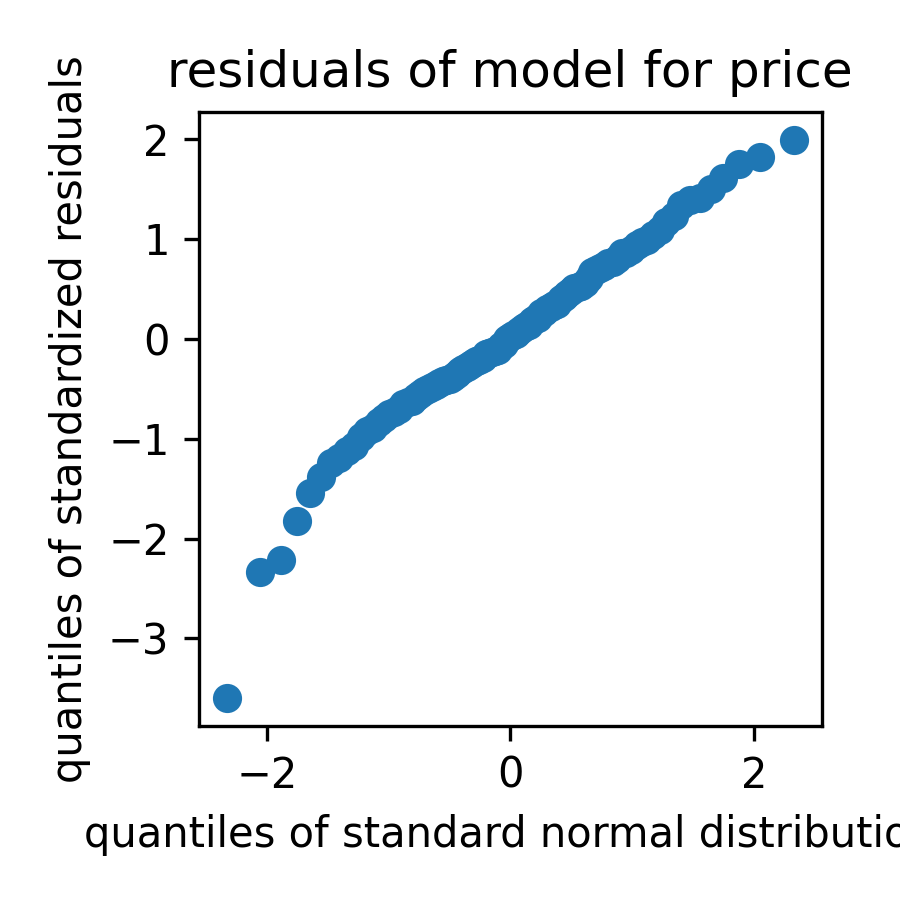
\includegraphics[width=\textwidth]{./images/qqplot_resz_price.png}
    \label{fig:qqplotreszprice}
  \end{subfigure}
  \begin{subfigure}[b]{0.32\textwidth}
    \centering
    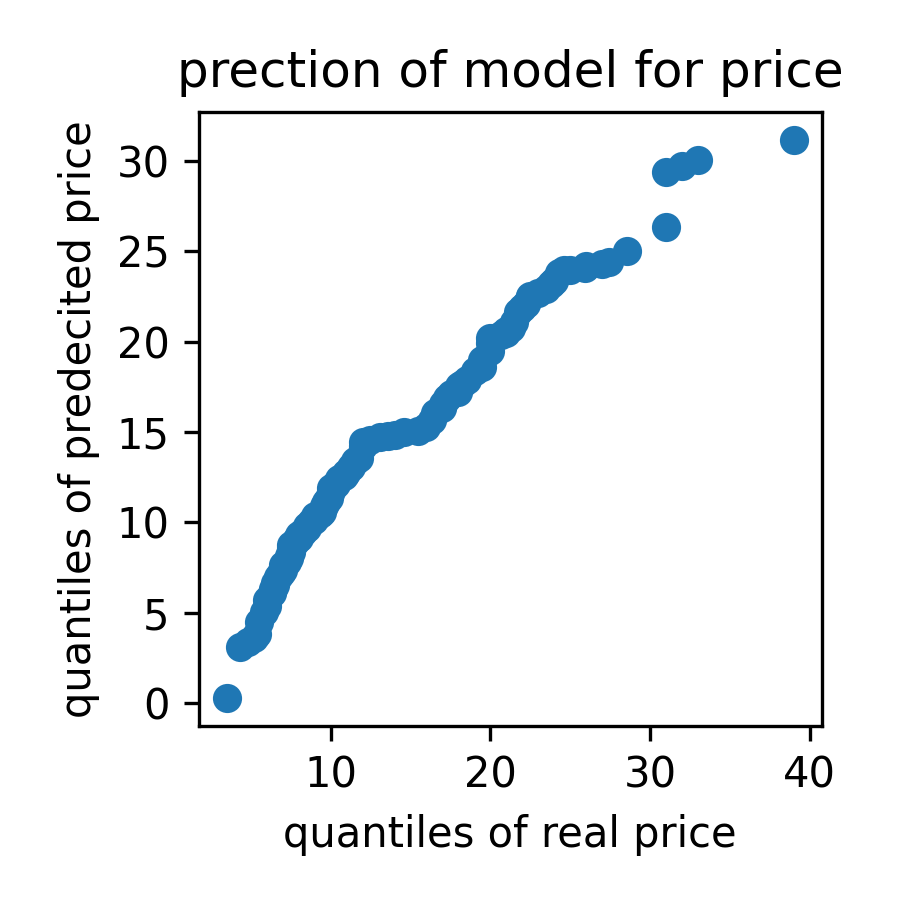
\includegraphics[width=\textwidth]{./images/qqplot_yyhat_price.png}
    \label{fig:qqplotyyhatprice}
  \end{subfigure}
  \begin{subfigure}[b]{0.32\textwidth}
    \centering
    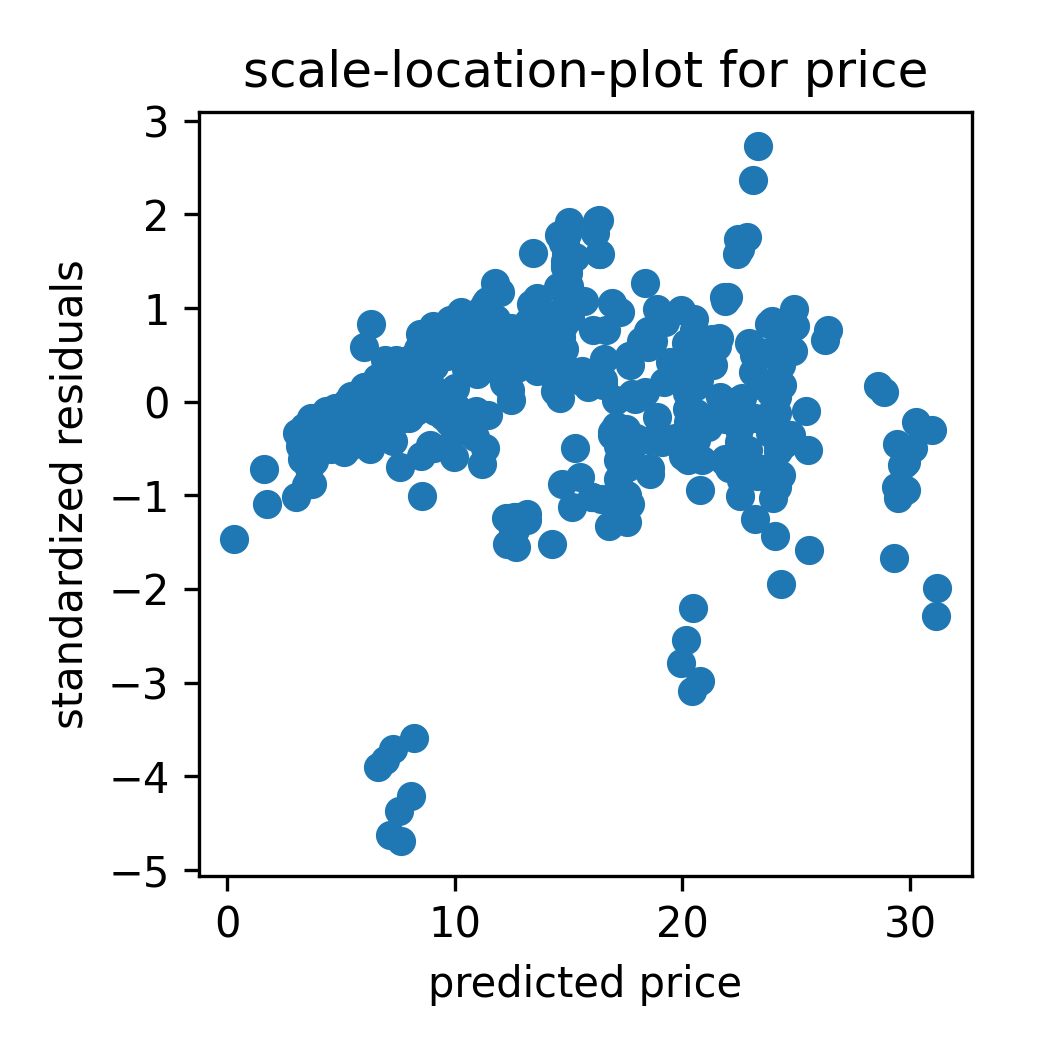
\includegraphics[width=\textwidth]{./images/scalelocationplot_price.png}
    \label{fig:scalelocationplotprice}
  \end{subfigure}

  \begin{subfigure}[b]{0.32\textwidth}
    \centering
    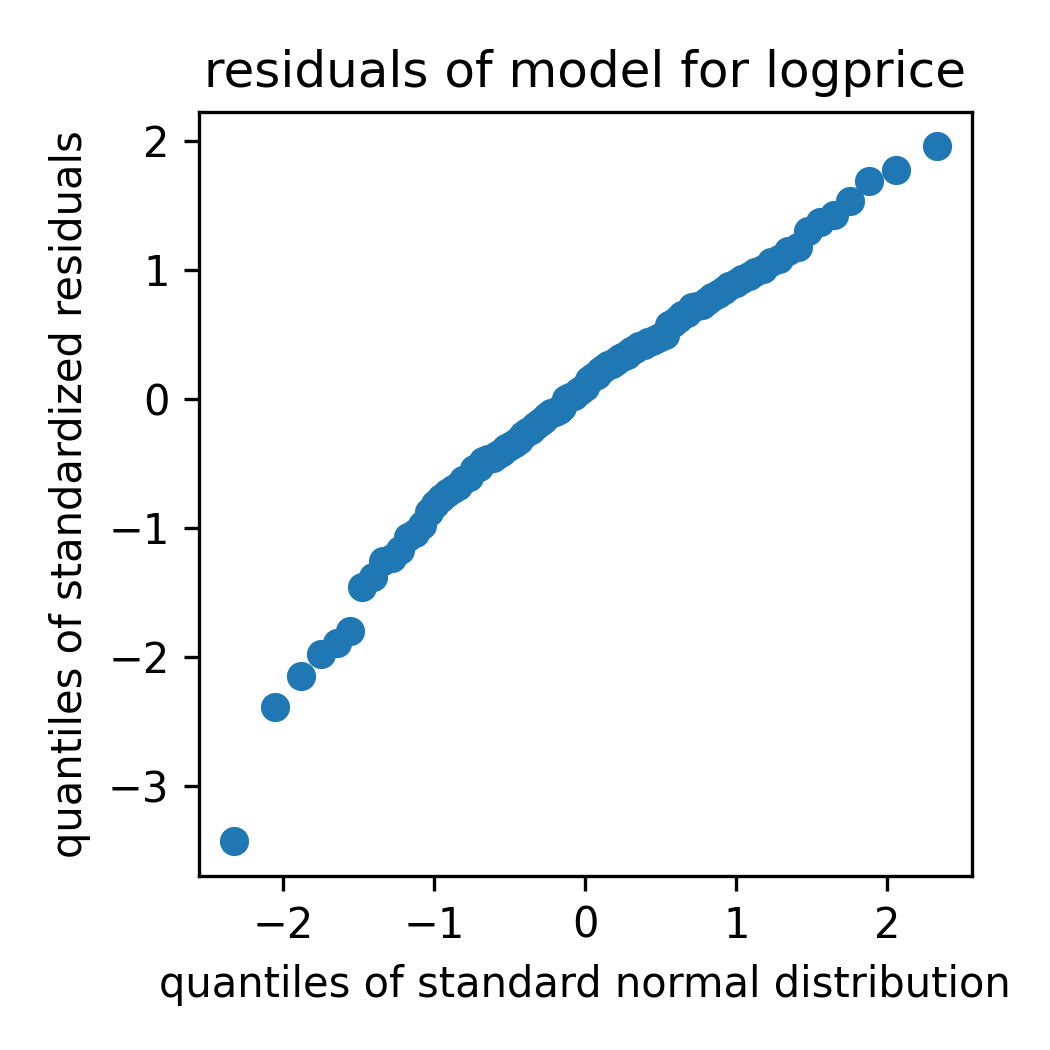
\includegraphics[width=\textwidth]{./images/qqplot_resz_logprice.png}
    \label{fig:qqplotreszlogprice}
  \end{subfigure}
  \begin{subfigure}[b]{0.32\textwidth}
    \centering
    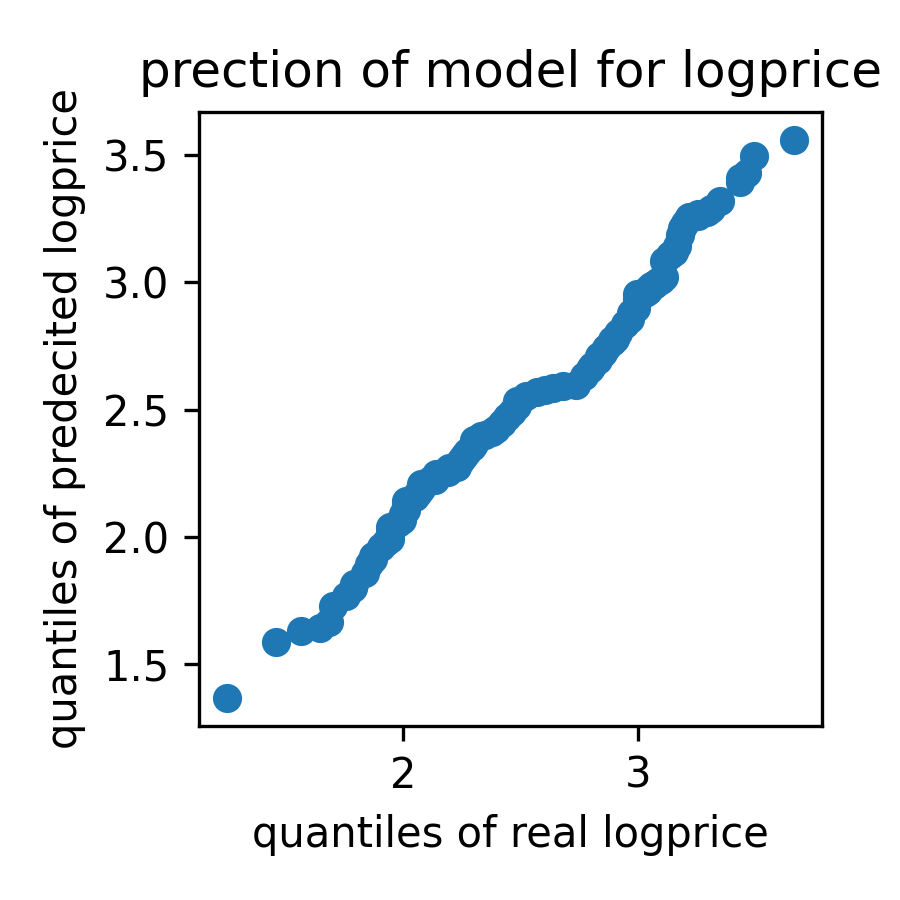
\includegraphics[width=\textwidth]{./images/qqplot_yyhat_logprice.png}
    \label{fig:qqplotyyhatlogprice}
  \end{subfigure}
  \begin{subfigure}[b]{0.32\textwidth}
    \centering
    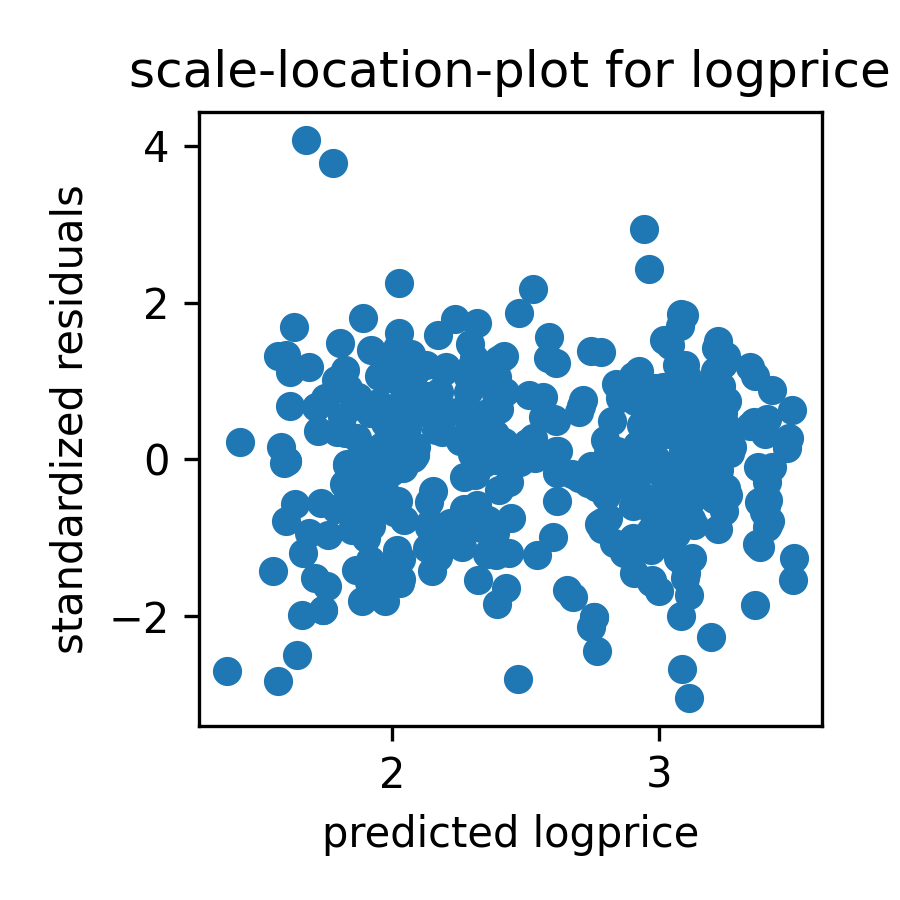
\includegraphics[width=\textwidth]{./images/scalelocationplot_logprice.png}
    \label{fig:scalelocationplotlogprice}
  \end{subfigure}
  \caption{q-q-plots comparing quantiles of standardized residuals with standard normal distribution and predicted values with real values, scale-location-plots for relationship between predicted value and standardized residuals.}
  \label{fig:pricevslogprice}
\end{figure}

As Figure~\ref{fig:pricevslogprice} shows, the residuals of the logprice model are closer to a normal distribution than those of the model with price as the dependent variable, because the line of points in the leftmost two q-q-plots is straighter for logprice. Also when predicting logprice instead of price, predicted values and real values seem to share a more similar distribution, as the middle two q-q-pots show. Also there seems to be a curvilinear relationship between predicted values and residuals when using price directly, which does not seem to be the case when using logprice. Finally also the adjusted $R^2$ value is higher for the logprice model ($R^2 = 0.962$) than for the price model ($R^2 = 0.939$), which suggests a better prediction. Therefore we go with the logprice as our dependent variable.

\subsection{best subset selection}

With our 8 predictor variables, best subset selection is performed to determine which model can predict the logprice best.
In total, 255 models ($= \sum_{i=1}^8{\choose{8}{i}} = 2^8-1$) have been fitted in iterations $i \in \{1,\dots,8\}$ to the data. Technically the number of predictors k used for models in iteration $i$ was not always the same, since categorical variables were split up into two dichotomous variables each (dummy coding), before performing model fitting. The models of each iteration were then sorted for their BIC and AIC values and the best value from each iteration $i$ can be seen in Table \ref{tab:subsetselection}

\begin{table}[ht]
  \centering
  \captionabove{Best subset selection: lowest AIC and BIC in each iteration and the respective model predictors added on top of predictors in all table cells above}
  \label{tab:subsetselection}
  \begin{tabular}{c|cccc}
    i & AIC              & BIC              & predictors       & models calculated \\
    \hline
    1 & 213.46           & 225.71           & model            & 8                 \\
    2 & -215.15          & -198.82          & age              & 28                \\
    3 & -414.14          & -393.73          & mileage          & 56                \\
    4 & -564.22          & -535.65          & transmission     & 70                \\
    5 & -651.78          & -619.12          & engineSize       & 56                \\
    6 & -706.25          & \textbf{-665.42} & fuelType         & 28                \\
    7 & \textbf{-706.41} & -661.51          & fuel consumption & 8                 \\
    8 & -706.35          & -657.37          & tax              & 1                 \\
  \end{tabular}
\end{table}

The AIC suggests that the model with 7 predictor variables (all but tax) is the best, while the BIC wants us to stop at iteration 6 and rises again for $i\ge7$. So the BIC suggests that in addition to tax, also fuel consumption should be excluded from the final model.
We will decide for the model the BIC suggests, which will include the predictors: model, age, mileage, transmission, engineSize and fuelType.

\subsection{final model}

Table \ref{tab:finalregression} shows the regression coefficients and their confidence intervals for the final model with 6 predictors (technically 9, if we count the dummy variables as single predictors). The model exhibits an adjusted $R^2$ value of 0.962 which is quite impressive and signifies a very good model fit. The predictor can explain 96.2\% of the variation in the logarithmic price. The good model fit can also be seen in the scatter plot in Figure~\ref{fig:finalmodel1} exhibiting a strong linear relationship between predicted logprice and real logprice. Figure~\ref{fig:finalmodel2} also shows that the residuals are spread out quite evenly, which is good.

\begin{figure}[htb]
  \centering
  \begin{subfigure}[b]{0.48\textwidth}
    \centering
    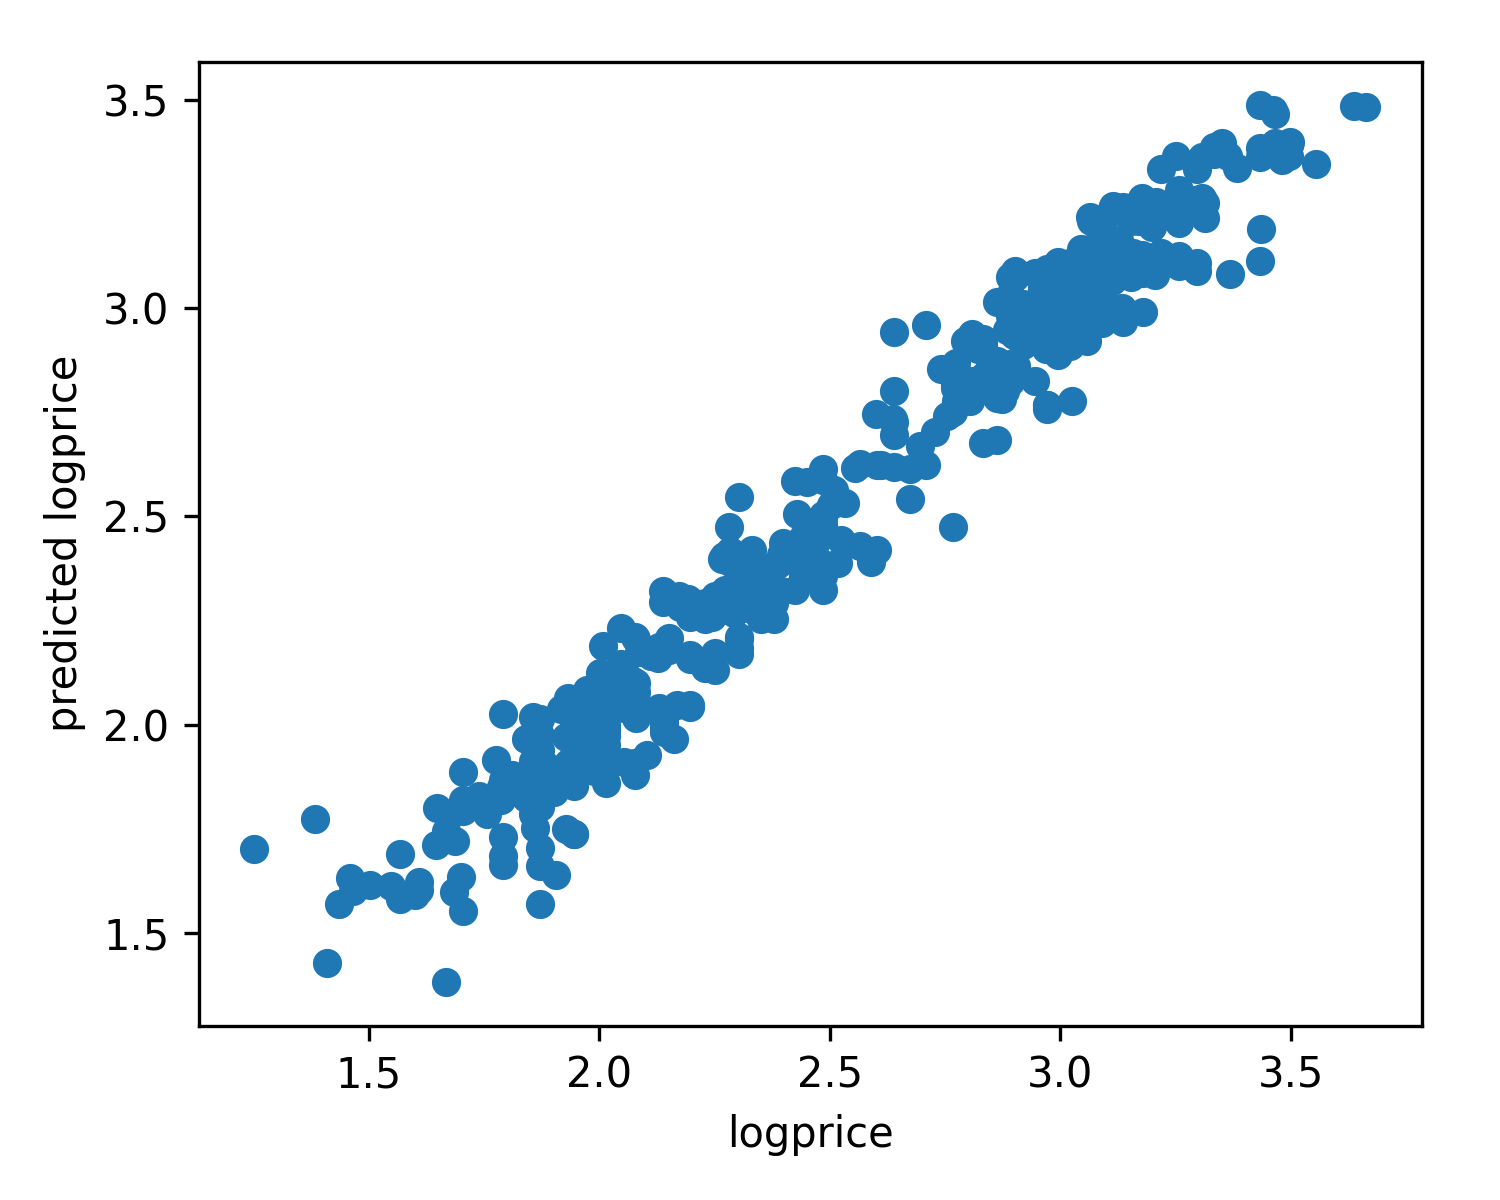
\includegraphics[width=\textwidth]{./images/finalmodel1.png}
    \caption{predicted logprice and real logprice}
    \label{fig:finalmodel1}
  \end{subfigure}
  \begin{subfigure}[b]{0.48\textwidth}
    \centering
    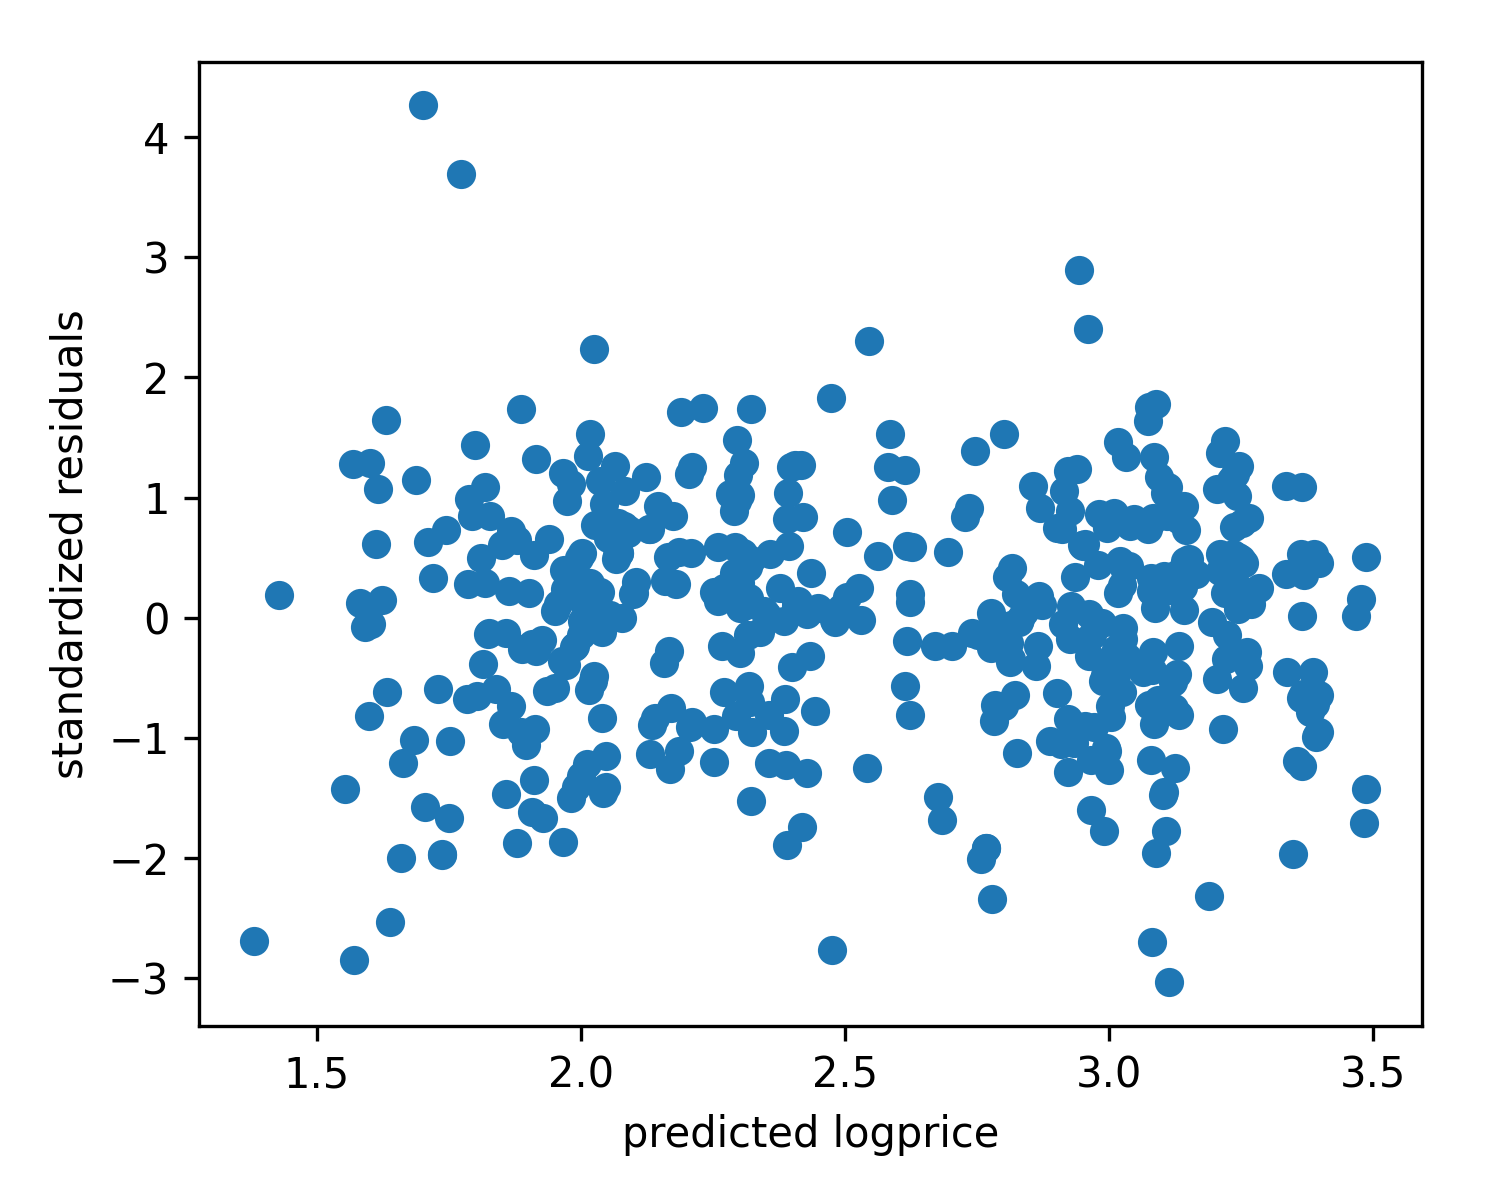
\includegraphics[width=\textwidth]{./images/finalmodel2.png}
    \caption{predicted logprice and standardized residuals}
    \label{fig:finalmodel2}
  \end{subfigure}
  \caption{plots for the final model with the lowest BIC}
  \label{fig:modelfit}
\end{figure}


All regression coefficients differ from 0 significantly since their 95\%-confidence intervals ($[CI_l, CI_u]$) do not contain 0.
We will now interpret the coefficients and their meaning for the real price, not the logprice.
The intercept of $\hat{\beta}_0 = 2.6160 = ln(13.681)$ tells us that the model assumes, for a Passat with Manual Transmission and Diesel an average price of 13,681 GPB, all other predictors held 0 (which is obviously not possible, only electric cars have an engineSize of 0 liters).

\begin{table}[ht]
  \centering
  \captionabove{The final regression model predicting logprice}
  \label{tab:finalregression}
  \begin{tabular}{c|cccc}
                            & $\hat{\beta}_j$ & $SE(\hat{\beta}_j)$ & $CI_l$ & $CI_u$ \\
    \hline
    intercept               & 2.6160          & 0.056               & 2.506  & 2.726  \\
    model: TRoc             & 0.1534          & 0.018               & 0.118  & 0.188  \\
    model: Up               & -0.5180         & 0.024               & -0.566 & -0.470 \\
    age                     & -0.0884         & 0.004               & -0.096 & -0.081 \\
    mileage                 & -0.0058         & 0.000               & -0.006 & -0.005 \\
    transmission: Automatic & 0.1221          & 0.019               & 0.085  & 0.159  \\
    transmission: Semi-Auto & 0.1180          & 0.018               & 0.083  & 0.153  \\
    engine size             & 0.2865          & 0.029               & 0.229  & 0.344  \\
    fuelType: Petrol        & 0.1227          & 0.020               & 0.084  & 0.161  \\
    fuelType: Hybrid        & 0.4623          & 0.037               & 0.389  & 0.535  \\
  \end{tabular}
\end{table}

A T-Roc seems to cost about 15.34\% more on average than Passat, while the model Up sells for less then half of a Passats price on average ($\hat{\beta} = -51.80\%$). An additional year of age seems to lower a cars price by almost 9\% ($\hat{\beta} = -8.84\%$). It is the second strongest predictor of a cars value (after model). Additional mileage also reduces a cars price: each additional 1000 miles on a car lower its value by approximately 0.58\%. Cars with
automatic or semi-automatic transmission sell for 12.21\% or 11.80\% more than cars with manual transmission according to the model. Mind that this holds for all other variables held constant, so the huge amount of cheap Up models that all just come with manual transmission cannot be the reason for this.
Engine size also matters: each additional liter of engine capacity increases a cars price by 28.65\%. The least important predictor is the fuel type. Not that it would not matter by itself, but the other predictors already explain a lot of variance so it was added last to the model in best subset selection.
Diesel cars are the cheapest. Compared to Diesel, the model predicts that petrol cars cost 12.27\% more and hybrid cars even 46.23\% more.
All percentages provided, have to be viewed in the light of their respective confidence intervals depicted in Table \ref{tab:finalregression}.

\subsection{Summary}

The question of this report was to determine which factors influence the price of VW-cars of the 3 popular types Passat, T-Roc and Up. For this, multiple linear regression was used. The data for the price and 8 predictor variables of 438 cars originated from the british car platform "Exchange and Mart", where mainly used cars are sold. In our analysis we found that it is more beneficial to predict the logarithmic price by the independent variables, than using the price directly. This also makes for a good interpretation of regression coefficients in terms of percentual changes. We found that in comparison to Passats, cars of the type Up sold for 51.80\% less and T-Rocs for about 15.34\% more. As they are totally different products, it does not come as a surprise that the car type was the strongest predictor of the price.
Cars seem to be depriciating assets, as every year of age decreases the value of cars in the data set by about 8.84\% on average. Also every 1000 miles put on a car, result in a loss of about 0.58\% of its worth. A reason could be, that an aging car requires more costly repairs and consumers mostly crave shiny new cars.
Also we found that having Automatic or Semi-Automatic transmission can increase a cars price by more than 10\% in comparison to manual transmission. Both features are associated with additional electronics and newer technology, so the price jump makes sense. \\
The engine size also matters, as our final regression model indicates that every liter of engine volume in connected to a price increase of 28.65\%. Apparently consumers are willing to pay more, for a more powerful car. Reasons might include fun while driving or a better sense of security by sharper handling.
Finally the weakest predictor for a cars price was the fuel type. In comparison to Diesel cars, Petrol cars are predicted to be worth roughly 12\% more and Hybird cars even 46\% more. This could be, because the Hybrid technology is still quite new and not many cars use it (only 2.9\% of cars in the data set).
The predictors fuel consumption and tax seem not to have great value for the prediction of car prices when added on top of the predictors mentioned on top and did not make it into the final model that resultet from best subset selection with respect to the BIC. All other predictors were significanctly different from 0 under $\alpha = 0.05$.
In total the model was able to explain more than 96\% in the variance of the logarithmic car price. This indicates a very strong model, which can quite accurately predict the value of an individual car. Sadly this is limited to VW cars of the 3 types present in the dataset, We would not recommend using this model for serious applications regarding totally different vehicles. \\
It has to be mentioned, that the multiple regression model coefficients each explain additional variance on top of the others. This does not mean though that they are truely the reasons for the difference in price. There could be covariates that we do not know about. For example consumers might be willing to pay more for a faster car which coincides with large engine size, so that engine size becomes a positive predictor. This does not mean however that the engine size must matter at all to the customer. Also we did not take into account interactions between the variables. For example it could be, that for a Passat automatic transmission is desirable and increases the price, while T-Roc buyers would value manual transmission more.
With only 438 objects in the data set we would not recommend adding interaction predictors though, because they would likely turn out irrelevant in best subset selection anyway and would not make a significant change.
Applications for the regression model might include decision systems for car dealerships or a web-browser extension that rates how good of a deal a certain offer on a website is. For future analysis an inclusion of more datapoints from more models and brands would be a sensible thing to do. To not inflate the car model as a predcitor, it could make sense to cluster different car models by their overall type like SUV, sportscar or small car.
In total we can be happy with the results and regard the prediction of car prices as quite successful.

\newpage
\addcontentsline{toc}{section}{Bibliography}
\renewcommand\refname{Bibliography}
\bibliographystyle{plainnat}
\bibliography{references}
\end{document}
